\section{Properties of photons}
If we have a decay of radiation
\begin{equation}
  E^{(+)}(t) = E_0e^{-2\pi i \nu_0t}e^{-\frac{\kappa}{2}t}
\end{equation}

\noindent and take its Fourier transform,  we get a Lorentzian, with an
intensity

 \begin{equation}
   \iabsSquared{f(\nu)} = \frac{4\iabs{E_0}^2}{\kappa^2 + \iabsSquared{4\pi(\nu_0 - \nu)}}.
 \end{equation}

 \begin{framed}\noindent

   It has a half-width of
   \begin{equation}
     \Delta\nu = \frac{\kappa}{2\pi},
   \end{equation}
   \noindent and since $ \Delta t = \kappa^{-1} $, we get the relationship

  \begin{equation}
    \Delta\nu\Delta t \approx \frac{1}{2\pi}
  \end{equation}

\end{framed}

 \subsection{Emission and line broadening}
 Classically,   we   have   en   ensembled  of   atom,   the   relaxing
 \iket{2}\ira\iket{1}.   If   we  hit   particles  to  take   away  the
 `unradiated' energy,  the relaxation  terminates, and atoms  emit only
 part  of the  full energy  $ \hbar\omega_{21}  $. Because  this is  an
 ensembled, on  average the energy  $ \hbar\omega_{21} $ will  still be
 emitted, just with a smaller $ \Delta t $, so the line broadens.

 Quantum  mechanically, we  cannot emit  `parts' of  $ \hbar\omega_{21}
 $. Either the photon is emitted,  or the photon is not. \red{Absurdly,
   if  tha atom  has been  emitting for  a certain  time, and  then the
   energy is  taken away (say during  a collision), then it  is free to
   \textbf{track  back}  and not  release  the  photon, or  release  it
   fully.}

 \subsection{Classical vs Quantum pulses}
 Suppose that an atom  emits a photon of frequency $ hf  $ and we start
 catching it by a localised detector (or just leave it to interact with
 the environment, which implicitly performs measurements for us)
 \begin{itemize}
 \item \underline{Classically} the energy is spread out over space \ira
   \textbf{we never measure the total energy of the pulse};
 \item \underline{Quantum} the photon will  be absorbed or not absorbed
   at different  points in space.   Performing an average over  all the
   positions, we find an exponential decay with a vertical front.
 \end{itemize}

 Now,  when  emission  takes   place,  the  wavefunction  evolves  from
 $ \Psi_2\Phi_{\text{vacuum}} $ to

 \begin{equation}
   e^{-\frac{\Gamma}{2}t}\Psi_2\Phi_{\text{vacuum}} + \sqrt{1-e^{-\Gamma t}}\Psi_1\Phi_{\text{photon}(t)}.
 \end{equation}

 What is important here?
 \begin{itemize}
 \item Upon measurement,  the wavefunction collapses to one  of the two
   states: 1) either the atom is  still excited; 2) the photon has been
   emitted;
 \item As  the relaxation occurs, $  \Phi_{\text{photon}}(t) $ evolves,
   to have a smaller and smaller  `tail' in the atom. The change occurs
   over a time $ \Gamma^{-1} $.
   \begin{framed}\noindent
     When  the atom  gives  all  its excitation  energy  away during  a
     collision and  nothing is  left to the  radiation field,  the atom
     need not “reel back” any field because, until that moment, no real
     emission took place. The latter emission happened only virtually –
     whatever that might mean!
   \end{framed}
 \item If  we leave  the system  for long enough,  it will,  by itself,
   transfer   irreversibly  to   state  $   \Psi_1\Phi_\text{photon}  $
   (normally quantum mechanics is reversible, as long as measurement is
   not made);
 \item The photon has a size
   \begin{equation}
     cT = \frac{c}{\Gamma}.
   \end{equation}
   \noindent This extension explains interference effects
   \begin{framed}\noindent
     The photon is spread  over space \textbf{before} measurement, with
     a distribution:
     \begin{equation}
       \iaverage{\hat{E}^{(-)}(\mathbf{r},t)\hat{E}^{(+)}(\mathbf{r},t)},
     \end{equation}
     \noindent  \red{and  the  probability  of  detectors  response  is
       propotional to it}.

     \red{\textbf{Upon each measurement the photon will be localised in
         a single space, as the wavefunction collapses.}} Two important
     errors are:
     \begin{itemize}
     \item The photon is not localised  before measurement - it's not a
       particle,  it's   a  wavefunciton   with  collapses   only  upon
       detection;
     \item The photons energy is not spread out - it's not a wave, it's
       a wavefunction.
     \end{itemize}
   \end{framed}

 \item Photons are never split \ira  in this case we would have photons
   of  energy  $  \frac{1}{2}hf  $,  which  would  dissapear  from  the
   observable world, as they have no atoms to be absorbed with.
 \item For interference we need two beams from the same source, so that
   phase fluctuations are the same - same as in the master beam.

\begin{framed}\noindent
  But what if now, we measure over a timescale \red{of the order of the
    coherence time}, preventing  washing out of the  pattern?  This was
  done  with  lasers (enough  power  to  have  many photons  for  clear
  interference) and an interference pattern was setup.
\end{framed}

\item A really cool way to measure interference patterns with very weak
  sources, is to take two beams, and beam split each one.
  \begin{itemize}
  \item   The  stronger   beams   should  intefere   on  a   controlled
    detector. The  interference pattern will constantly  change (as the
    phase changes randomly in each beam).  We pick on such pattern, and
    produced a square pulse \textbf{only} when it is formed;
  \item This pulse  is used to open a shutter  on another screen, where
    the weaker beams are sent through.   Thus, we will be building up a
    pattern of  the two beams at  a fixed phase, even  though they come
    from two sources!
  \end{itemize}
  Note  that for  such weak  intensities, the  photon picture  of light
  completely  fails  -  if  they  were  partciles  then  its  extremely
  improbable that both will be passing throught the shutter at the same
  time to interfere  with one another.  Here light behaves  more like a
  wave.
\end{itemize}

 \subsection{More about photons}
 We can  also apply  laser pulses  to form  superpositions of  2 atomic
 states. It  is possible for the  system to transition into  one energy
 level simultaneously.   \red{The emitted photon will  have elements of
   both excited atomic states - this  will show up as the photon having
   two frequencies!}


\begin{figure}[h]
  \centering%
  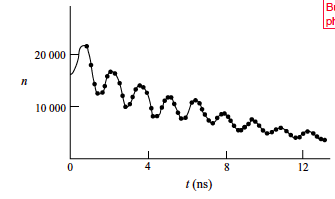
\includegraphics[height=6cm]{photon_beating}
  \caption{\small Suppose  that we create  a superposition in  the atom
    $ \frac{\iket{1}+\iket{2}}{\sqrt{2}} $. Then there are two possible
    ways for the atom to decay to the ground energy state and create an
    outgoing photon.  When we measure the intensity of the photon, with
    the  outgoing detector,  the photons  1\ira0 and  2\ira0 components
    will interfere to  produed beatings. The photon  is thus imprinting
    the  full information  of the  atomic excitation.   \red{Oh, did  I
      mention  this is  a  single photon?   Classically  this would  be
      impossible to do with a single photon.}}
\end{figure}

\noindent

\begin{itemize}
\item   \textbf{Parametric   fluorescence:}  during   parametric   down
  conversion  in a  non-linear  medium, a  single photon  spontanesouly
  decays into two more (idler  and signal), abiding energy and momentum
  conservation:

  \begin{equation}
    \begin{aligned}
      \hbar(\omega_p) & = \hbar(\omega_i + \omega_s);\\
      \hbar\mathbf{k_p} & = \hbar(\mathbf{k_i} + \mathbf{k_s}).
    \end{aligned}
  \end{equation}

  \noindent The emitted  photons become entangled and will  have a very
  strong  correlation  in  terms   of  total  energy  and  simultaneous
  mesasurement.

  Such fluorescence photons are good to  use as single photon sources -
  registering  the  idler   photon,  we  can  be  100\%   sure  that  a
  corresponding signal photon is flying in a specific direction
\item Now  consider forming an  interference pattern with  photons. The
  clarity of the interference pattern depends on the uncertainty of the
  phase,  $  \Delta\phi $.   The  phase  and  photon number  abide  the
  relationship
  \begin{equation}
    \Delta n\Delta\phi \ge\frac{1}{2},
  \end{equation}
  \noindent  so  surely  with   decreasing  photon  number  (decreasing
  $ \Delta n $), the phase should diverge and wash out interference! \iRa In
  reality  the  phase  uncertainty  accumulates  in  the  vacuum  state
  \iket{0}, which does not contribute to the interferene pattern.
\item To ensure good matching of  frequencies from two sources, one can
  measure beats  in interference  patterns, and  only open  the shutter
  when the beats oscillate slowly (good frequency matching).
\end{itemize}

 \subsection{Photon bunching}
 We begun with discussing that  when observing stars.  We use something
 similar to an  interferometer, and pick up an  interference pattern on
 the telescope screen.

 Now consider a second light source  (different part of the planet). It
 will fly in at an ever small different angle, and \textbf{its' pattern
   will be shifted, relative to the initial one}. An overlap will occur
 if we increse the separation  of the telescope mirrors (increasing the
 phase  difference  between the  patterns).   \red{This  is called  the
   coherence length - separation at which interference vanishes}

\begin{framed}\noindent
  Probability that  two photons  arrive at the  same place  shrotly one
  after another  i.e.  $ \tau  < t_{\text{coh}} $  is higher than  if they
  arrive with a larger time delay $ \tau > t_\text{coh}. $

  \textbf{\Huge This is exactly analogous to the coherene length above,
    except in time!}
\end{framed}

If one thinks in the photon  pitcture, this implies that photon sources
communicate    with    each    other     to    release    photons    in
pairs. \red{\textbf{But this is seriously  wrong!} It is actually do do
  with inteference  between the  waves emitted by  completely different
  atoms!}

\subsection{Types of light}
\begin{framed}\noindent
  \red{\textbf{Coherence  volume}}  \red{or  time} is  over  which  the
  \textbf{instantaenous} phase does not change significantly within it.

  The    photon    number   is    related    to    the   mode    volume
  $ V_\text{coherence} $. In experiments we must be working within this
  volume,  or within  the  related time  $ T  $,  over which  coherence
  persists. \red{If a  fraction of the volume (time)  is observed, then
    only a fraction of photons present are observed}
\end{framed}
\begin{enumerate}
\item \textbf{Thermal  light, is  formed of  partial waves  with random
    phases.}  The intensity fluctuates  in time.  \red{The bandwidth of
    scattered  light is  very  narrow}, giving  a  large $  \Delta  t $  for
  intensity correlation measurements.

  It  follows a  Bose einstein  distribution  which is  very broad  and
  \textbf{the photons are subject to bunching!}

\item  \textbf{Laser light}  has a  constant amplitude  (intensity) and
  follows a Poisson distribution, which  is much narrower than the Bose
  one for thermal light.

\begin{figure}[h]
  \centering%
  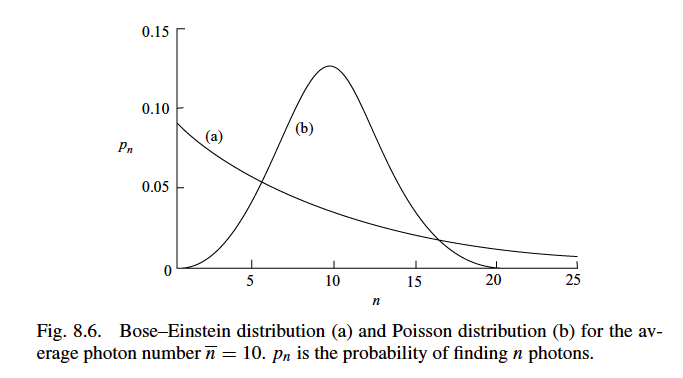
\includegraphics[height=6cm]{photon_distribution}
\end{figure}

\noindent

Laser light  does not  tend to  bunch (unlike  thermal light)  with the
coincidence  photon rate  being  the  same as  the  random  one -  same
probability  of  detecting photons  for  all  kinds of  different  time
delays.
\end{enumerate}

\subsection{Photon antibunching}
\begin{framed}\noindent
  Occurs with photons with a sharp photon number \iaverage{n}.
\end{framed}
So now consider  the case of a detector, which  accumulates over a time
(or volume) $ V_\text{obs} $. It has probability

  \begin{equation}\label{eqn:bookQO_1}
    t = \frac{V_\text{obs}}{V_\text{coh}}\eta,
  \end{equation}

  \noindent of  detecting a photon, which  depends on the ratio  of the
  observed to the coherence  volume (\textbf{recall that photon numbers
    are associated  with the  mode volume  $ V_\text{coh}  $, so  if we
    observe  a smaller  volume,  than  we register  a  fraction of  the
    photons.})

  The detector either detects or photon  (with probabiltiy $ t $) or it
  doesn't.  So  the probability  of transmitting  $ k  $ out  of $  n $
  photons follows a binomial distribution

  \begin{equation}
    \text{Prob(k photons)} = \imatrixcol{n}{k}t^{k}r^{n-k},
  \end{equation}

  \noindent which has a variance

  \begin{equation}
    \Delta k^2 = (1-t)\iaverage{k} \qquad (\equiv \iaverage{k^2} - \iaverage{k}^2).
  \end{equation}

  \noindent Now, look out!
  \begin{itemize}
  \item     The     lower      the     detection     probabulity     in
    Eq.~\eqref{eqn:bookQO_1}, due to shorter  integration time or lower
    efficiency, the large the variance $ \Delta k^2 $.
  \item If however we are able to  detect all photon in the mode volume
    $ V_\text{coh} $, then there should be no variance.
  \end{itemize}

\begin{framed}\noindent
  \red{Unlike with bunched light, where photon number is undefined, the
    ratio of random clicks to simulatneous clicks}

 \begin{equation}
   R = \frac{\Delta n^2 - \iaverage{n}}{\iaverage{n}^2},
 \end{equation}
 \noindent  \red{can  be  negative! \textbf{Negative  relative  to  the
     counts we  would measure outside the  coherence time/volume, where
     statistics were random.}}

 This is showing photon antibunching, whereby  photon do not tend to be
 simultaneously detected in the same coherence volume.

\end{framed}

Let us disuss this more fully
\begin{itemize}
\item Classically  the coincidence coutning rate  (simultaneous clicks)
  $ \propto I(t)I(t+\tau)  $, which has a maximum  at $ \tau = 0  $ (opposite of
  antibunching);
\item \textbf{Antibunching:} (Sub-)Poisson  statistics for \iaverage{n}
  \ira  0.  $  \Delta  n <  \iaverage{n}$.  \red{Only  when  we fire  single
    photons.};
\item  \textbf{Bunching:}  Poisson  statistics  for  \iaverage{n}  \ira
  $ \infty $. $ \Delta n > \iaverage{n} $.
\item
\end{itemize}

 \subsection{Creating antibunching}
 To create  a stream  of bullets  (which is not  how we  imagined light
 classically - we used to think of it as a wave)
 \begin{itemize}
 \item Use  atoms flying through cavity  \ira excite and allow  some of
   them  to relax  \ira then  measure  with an  ionisation detector  to
   recover photon statistics from the de-excited atom statistics;
 \item  Create electron  hole  pairs  and create  light  emission in  a
   controlled way;
 \end{itemize}

 \subsection{Squeezed light}
 Squeezed light has a $ \Delta x $ or $ \Delta p $ smaller than vacuum. The other
 component  is correspondingly  blown up.   These two  quantities arise
 when we rewrite the field

  \begin{equation}
    \mathbf{E}(\vec{r},t) = Ae^{i(\vec{k}\vec{r} - \omega t)} + A^{*}e^{-i(\vec{k}\vec{r} - \omega t)},
  \end{equation}

  The quantum mechanical description of the field is
  \[
    \hat{E} =  \hat{E}^{(+)} + \hat{E}^{(-)} =  e^{-i\omega t}\hat{a} +
    e^{i\omega t}\hat{a}\idagger,
  \]

  \noindent  \red{where  the amplitude  is  replaced  with the  quantum
    mechanical field  operators, telling  how many  photons are  in the
    field.} The energy of the field is

  \[
    \hat{H} = \hbar\omega\hat{a}\idagger\hat{a}
  \]

  \begin{framed}\noindent
    \begin{itemize}
    \item  Electric field  strength \iaverage{\hat{E}}  = 0  for states
      with  well defined  photon  number \iket{n}.   (The  $ \hat{a}  $
      operators raise and lower this number, so that the product of two
      different `kets' is 0.)
    \end{itemize}
  \end{framed}

  \noindent      in      terms      of      two      new      variables
  $ x = \mathcal{Re}{A}, p =\mathcal{Im}{A} $

  \begin{equation}
    E(\vec{r},t) = C\bigg[x\cos(\omega t - \vec{k}\vec{r}) + p\sin(\omega t - \vec{k}\vec{r})\bigg]
  \end{equation}

 \subsection{Phase distribution}
 Say we want to measure the phase distribution of the field

  \begin{equation}
    E(z,t) \propto \cos(\omega t - \phi - kz),
  \end{equation}

  \noindent which we rewrite

  \begin{equation}
    \begin{aligned}
      \cos(\phi)& \cos(\omega t - kz) &+ \sin(\phi)&\sin(\omega t - kz)\\
      \frac{x}{\sqrt{x^2+p^2}} & \cos(\omega t - kz) &+ \frac{p}{\sqrt{x^2+p^2}}&\sin(\omega t - kz)\\
    \end{aligned}.
  \end{equation}

\begin{framed}\noindent
  So by measuring the quadrates of the  field, we can map out the x and
  the  p components.   The  are multiple  ways of  describing  $ x,p  $
  distribution in  phase space  (where distance  from axis,  $ \rho  $, is
  amplitude, and angle, $ \phi $:
  \begin{itemize}
  \item Through the Q function
    \begin{equation}
      w(x,p) = \frac{1}{\pi}\iabsSquared{\bra{\psi}\ket{\alpha}},
    \end{equation}
    \noindent which looses some  information about the $ x $  and $ p $
    distribution, due to them being non commutable observables;
  \item Wigner function, which gives full information about the state
    \begin{equation}
      W(x,p) = \frac{1}{\pi}\int_{-\infty}^{\infty}e^{i2py}\psi(x-y)\psi^{*}(x+y)dy.
    \end{equation}
    \noindent This turns into the Q function, if we convolute it with a
    Gaussian, which smooths the function out.
  \end{itemize}
  )
\end{framed}

\newpage
